% !TeX spellcheck = cs_CZ
\documentclass[10pt]{scrartcl}
\usepackage[]{geometry}     %showframe
\geometry{
  paperwidth=7cm,
  paperheight=1.17cm,
  margin=1pt
}

\usepackage[usenames,x11names]{xcolor}
  \definecolor{beige}{rgb}{0.96, 0.96, 0.86}
  \definecolor{bazaar}{rgb}{0.6, 0.47, 0.48}
  \definecolor{blue(pigment)}{rgb}{0.2, 0.2, 0.6}
  \definecolor{cadmiumgreen}{rgb}{0.0, 0.42, 0.24}
\usepackage{tikz}
  \usetikzlibrary{positioning}
\usepackage{pgfplots}
  \pgfplotsset{compat=newest}
\usepackage{amsmath}

\begin{document}
\noindent
  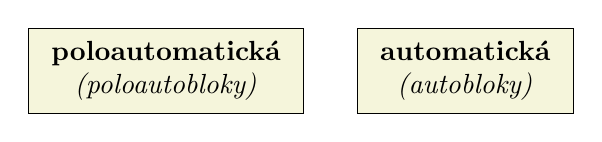
\begin{tikzpicture}[fill=beige, scale=1, every node/.style={scale=1}]
    \tikzstyle{nome}=[ %
%     draw, rectangle,
      anchor=west, 
      minimum width=7cm,
%      fill=yellow!30,
      outer sep=1,inner sep=0,
      node distance=12,
      text width=7cm
    ]
  %  \draw[help lines] (-1,-2) grid (6,3);
    \path (0,0)  node(a) [rectangle,draw,fill] 
                {\(\begin{array}{c} 
                    \text{\textbf{poloautomatická}} \\ \text{\emph{(poloautobloky)}}
                    \end{array}\)
                }
          (3.8,0) node(d) [rectangle,draw,fill] 
                {\(\begin{array}{c} 
                    \text{\textbf{automatická}} \\ \text{\emph{(autobloky)}}
                    \end{array}\)
                };
  \end{tikzpicture}
\end{document}